\documentclass[twoside]{book}

% Packages required by doxygen
\usepackage{fixltx2e}
\usepackage{calc}
\usepackage{doxygen}
\usepackage[export]{adjustbox} % also loads graphicx
\usepackage{graphicx}
\usepackage[utf8]{inputenc}
\usepackage{makeidx}
\usepackage{multicol}
\usepackage{multirow}
\PassOptionsToPackage{warn}{textcomp}
\usepackage{textcomp}
\usepackage[nointegrals]{wasysym}
\usepackage[table]{xcolor}

% Font selection
\usepackage[T1]{fontenc}
\usepackage[scaled=.90]{helvet}
\usepackage{courier}
\usepackage{amssymb}
\usepackage{sectsty}
\renewcommand{\familydefault}{\sfdefault}
\allsectionsfont{%
  \fontseries{bc}\selectfont%
  \color{darkgray}%
}
\renewcommand{\DoxyLabelFont}{%
  \fontseries{bc}\selectfont%
  \color{darkgray}%
}
\newcommand{\+}{\discretionary{\mbox{\scriptsize$\hookleftarrow$}}{}{}}

% Page & text layout
\usepackage{geometry}
\geometry{%
  a4paper,%
  top=2.5cm,%
  bottom=2.5cm,%
  left=2.5cm,%
  right=2.5cm%
}
\tolerance=750
\hfuzz=15pt
\hbadness=750
\setlength{\emergencystretch}{15pt}
\setlength{\parindent}{0cm}
\setlength{\parskip}{3ex plus 2ex minus 2ex}
\makeatletter
\renewcommand{\paragraph}{%
  \@startsection{paragraph}{4}{0ex}{-1.0ex}{1.0ex}{%
    \normalfont\normalsize\bfseries\SS@parafont%
  }%
}
\renewcommand{\subparagraph}{%
  \@startsection{subparagraph}{5}{0ex}{-1.0ex}{1.0ex}{%
    \normalfont\normalsize\bfseries\SS@subparafont%
  }%
}
\makeatother

% Headers & footers
\usepackage{fancyhdr}
\pagestyle{fancyplain}
\fancyhead[LE]{\fancyplain{}{\bfseries\thepage}}
\fancyhead[CE]{\fancyplain{}{}}
\fancyhead[RE]{\fancyplain{}{\bfseries\leftmark}}
\fancyhead[LO]{\fancyplain{}{\bfseries\rightmark}}
\fancyhead[CO]{\fancyplain{}{}}
\fancyhead[RO]{\fancyplain{}{\bfseries\thepage}}
\fancyfoot[LE]{\fancyplain{}{}}
\fancyfoot[CE]{\fancyplain{}{}}
\fancyfoot[RE]{\fancyplain{}{\bfseries\scriptsize Generated by Doxygen }}
\fancyfoot[LO]{\fancyplain{}{\bfseries\scriptsize Generated by Doxygen }}
\fancyfoot[CO]{\fancyplain{}{}}
\fancyfoot[RO]{\fancyplain{}{}}
\renewcommand{\footrulewidth}{0.4pt}
\renewcommand{\chaptermark}[1]{%
  \markboth{#1}{}%
}
\renewcommand{\sectionmark}[1]{%
  \markright{\thesection\ #1}%
}

% Indices & bibliography
\usepackage{natbib}
\usepackage[titles]{tocloft}
\setcounter{tocdepth}{3}
\setcounter{secnumdepth}{5}
\makeindex

% Hyperlinks (required, but should be loaded last)
\usepackage{ifpdf}
\ifpdf
  \usepackage[pdftex,pagebackref=true]{hyperref}
\else
  \usepackage[ps2pdf,pagebackref=true]{hyperref}
\fi
\hypersetup{%
  colorlinks=true,%
  linkcolor=blue,%
  citecolor=blue,%
  unicode%
}

% Custom commands
\newcommand{\clearemptydoublepage}{%
  \newpage{\pagestyle{empty}\cleardoublepage}%
}

\usepackage{caption}
\captionsetup{labelsep=space,justification=centering,font={bf},singlelinecheck=off,skip=4pt,position=top}

%===== C O N T E N T S =====

\begin{document}

% Titlepage & ToC
\hypersetup{pageanchor=false,
             bookmarksnumbered=true,
             pdfencoding=unicode
            }
\pagenumbering{alph}
\begin{titlepage}
\vspace*{7cm}
\begin{center}%
{\Large Game\+Tree\+Core \\[1ex]\large 1.\+0 }\\
\vspace*{1cm}
{\large Generated by Doxygen 1.8.14}\\
\end{center}
\end{titlepage}
\clearemptydoublepage
\pagenumbering{roman}
\tableofcontents
\clearemptydoublepage
\pagenumbering{arabic}
\hypersetup{pageanchor=true}

%--- Begin generated contents ---
\chapter{Namespace Index}
\section{Packages}
Here are the packages with brief descriptions (if available)\+:\begin{DoxyCompactList}
\item\contentsline{section}{\mbox{\hyperlink{namespace_hus}{Hus}} }{\pageref{namespace_hus}}{}
\end{DoxyCompactList}

\chapter{Hierarchical Index}
\section{Class Hierarchy}
This inheritance list is sorted roughly, but not completely, alphabetically\+:\begin{DoxyCompactList}
\item \contentsline{section}{Game\+Tree\+Core.\+I\+Child\+Selection\+Service}{\pageref{interface_game_tree_core_1_1_i_child_selection_service}}{}
\begin{DoxyCompactList}
\item \contentsline{section}{Game\+Tree\+Core.\+Child\+Selection\+Service\+Alpha\+A\+M\+AF}{\pageref{class_game_tree_core_1_1_child_selection_service_alpha_a_m_a_f}}{}
\begin{DoxyCompactList}
\item \contentsline{section}{Game\+Tree\+Core.\+Child\+Selection\+Service\+A\+M\+AF}{\pageref{class_game_tree_core_1_1_child_selection_service_a_m_a_f}}{}
\item \contentsline{section}{Game\+Tree\+Core.\+Child\+Selection\+Service\+U\+CT}{\pageref{class_game_tree_core_1_1_child_selection_service_u_c_t}}{}
\end{DoxyCompactList}
\item \contentsline{section}{Game\+Tree\+Core.\+Child\+Selection\+Service\+R\+A\+VE}{\pageref{class_game_tree_core_1_1_child_selection_service_r_a_v_e}}{}
\item \contentsline{section}{Game\+Tree\+Core.\+Child\+Selection\+Service\+Silver\+Alpha\+A\+M\+AF}{\pageref{class_game_tree_core_1_1_child_selection_service_silver_alpha_a_m_a_f}}{}
\end{DoxyCompactList}
\item \contentsline{section}{Game\+Tree\+Core.\+I\+Final\+Child\+Selection\+Service}{\pageref{interface_game_tree_core_1_1_i_final_child_selection_service}}{}
\begin{DoxyCompactList}
\item \contentsline{section}{Game\+Tree\+Core.\+Final\+Child\+Selection\+Service\+M\+AX}{\pageref{class_game_tree_core_1_1_final_child_selection_service_m_a_x}}{}
\item \contentsline{section}{Game\+Tree\+Core.\+Final\+Child\+Selection\+Service\+R\+O\+B\+U\+ST}{\pageref{class_game_tree_core_1_1_final_child_selection_service_r_o_b_u_s_t}}{}
\item \contentsline{section}{Game\+Tree\+Core.\+Final\+Child\+Selection\+Service\+S\+E\+C\+U\+RE}{\pageref{class_game_tree_core_1_1_final_child_selection_service_s_e_c_u_r_e}}{}
\end{DoxyCompactList}
\item \contentsline{section}{Game\+Tree\+Core.\+I\+Game\+Tree\+Node}{\pageref{interface_game_tree_core_1_1_i_game_tree_node}}{}
\end{DoxyCompactList}

\chapter{Class Index}
\section{Class List}
Here are the classes, structs, unions and interfaces with brief descriptions\+:\begin{DoxyCompactList}
\item\contentsline{section}{\mbox{\hyperlink{class_game_tree_core_1_1_child_selection_service_alpha_a_m_a_f}{Game\+Tree\+Core.\+Child\+Selection\+Service\+Alpha\+A\+M\+AF}} \\*A child selection service based on the alpha A\+M\+AF algorithm. }{\pageref{class_game_tree_core_1_1_child_selection_service_alpha_a_m_a_f}}{}
\item\contentsline{section}{\mbox{\hyperlink{class_game_tree_core_1_1_child_selection_service_a_m_a_f}{Game\+Tree\+Core.\+Child\+Selection\+Service\+A\+M\+AF}} \\*A child selection service based on the A\+M\+AF algorithm. This is a special case of the alpha A\+M\+AF version (alpha = 1). }{\pageref{class_game_tree_core_1_1_child_selection_service_a_m_a_f}}{}
\item\contentsline{section}{\mbox{\hyperlink{class_game_tree_core_1_1_child_selection_service_r_a_v_e}{Game\+Tree\+Core.\+Child\+Selection\+Service\+R\+A\+VE}} \\*A child selection service based on the R\+A\+VE algorithm. }{\pageref{class_game_tree_core_1_1_child_selection_service_r_a_v_e}}{}
\item\contentsline{section}{\mbox{\hyperlink{class_game_tree_core_1_1_child_selection_service_silver_alpha_a_m_a_f}{Game\+Tree\+Core.\+Child\+Selection\+Service\+Silver\+Alpha\+A\+M\+AF}} \\*A child selection service based on the alpha A\+M\+AF algorithm from David Silver. }{\pageref{class_game_tree_core_1_1_child_selection_service_silver_alpha_a_m_a_f}}{}
\item\contentsline{section}{\mbox{\hyperlink{class_game_tree_core_1_1_child_selection_service_u_c_t}{Game\+Tree\+Core.\+Child\+Selection\+Service\+U\+CT}} \\*A child selection service based on the U\+CT algorithm. This is a special case of the alpha A\+M\+AF version (alpha = 0). }{\pageref{class_game_tree_core_1_1_child_selection_service_u_c_t}}{}
\item\contentsline{section}{\mbox{\hyperlink{class_game_tree_core_1_1_final_child_selection_service_m_a_x}{Game\+Tree\+Core.\+Final\+Child\+Selection\+Service\+M\+AX}} }{\pageref{class_game_tree_core_1_1_final_child_selection_service_m_a_x}}{}
\item\contentsline{section}{\mbox{\hyperlink{class_game_tree_core_1_1_final_child_selection_service_r_o_b_u_s_t}{Game\+Tree\+Core.\+Final\+Child\+Selection\+Service\+R\+O\+B\+U\+ST}} }{\pageref{class_game_tree_core_1_1_final_child_selection_service_r_o_b_u_s_t}}{}
\item\contentsline{section}{\mbox{\hyperlink{class_game_tree_core_1_1_final_child_selection_service_s_e_c_u_r_e}{Game\+Tree\+Core.\+Final\+Child\+Selection\+Service\+S\+E\+C\+U\+RE}} }{\pageref{class_game_tree_core_1_1_final_child_selection_service_s_e_c_u_r_e}}{}
\item\contentsline{section}{\mbox{\hyperlink{interface_game_tree_core_1_1_i_child_selection_service}{Game\+Tree\+Core.\+I\+Child\+Selection\+Service}} \\*Exposes a method to select a child node from a \mbox{\hyperlink{interface_game_tree_core_1_1_i_game_tree_node}{I\+Game\+Tree\+Node}}. }{\pageref{interface_game_tree_core_1_1_i_child_selection_service}}{}
\item\contentsline{section}{\mbox{\hyperlink{interface_game_tree_core_1_1_i_final_child_selection_service}{Game\+Tree\+Core.\+I\+Final\+Child\+Selection\+Service}} \\*Esposes a method to finally select a child node from a \mbox{\hyperlink{interface_game_tree_core_1_1_i_game_tree_node}{I\+Game\+Tree\+Node}}. }{\pageref{interface_game_tree_core_1_1_i_final_child_selection_service}}{}
\item\contentsline{section}{\mbox{\hyperlink{interface_game_tree_core_1_1_i_game_tree_node}{Game\+Tree\+Core.\+I\+Game\+Tree\+Node}} \\*Represents a node in a game tree. ~\newline
}{\pageref{interface_game_tree_core_1_1_i_game_tree_node}}{}
\end{DoxyCompactList}

\chapter{Namespace Documentation}
\hypertarget{namespace_game_tree_core}{}\section{Game\+Tree\+Core Namespace Reference}
\label{namespace_game_tree_core}\index{Game\+Tree\+Core@{Game\+Tree\+Core}}
\subsection*{Classes}
\begin{DoxyCompactItemize}
\item 
class \mbox{\hyperlink{class_game_tree_core_1_1_child_selection_service_alpha_a_m_a_f}{Child\+Selection\+Service\+Alpha\+A\+M\+AF}}
\begin{DoxyCompactList}\small\item\em A child selection service based on the alpha A\+M\+AF algorithm. \end{DoxyCompactList}\item 
class \mbox{\hyperlink{class_game_tree_core_1_1_child_selection_service_a_m_a_f}{Child\+Selection\+Service\+A\+M\+AF}}
\begin{DoxyCompactList}\small\item\em A child selection service based on the A\+M\+AF algorithm. This is a special case of the alpha A\+M\+AF version (alpha = 1). \end{DoxyCompactList}\item 
class \mbox{\hyperlink{class_game_tree_core_1_1_child_selection_service_r_a_v_e}{Child\+Selection\+Service\+R\+A\+VE}}
\begin{DoxyCompactList}\small\item\em A child selection service based on the R\+A\+VE algorithm. \end{DoxyCompactList}\item 
class \mbox{\hyperlink{class_game_tree_core_1_1_child_selection_service_silver_alpha_a_m_a_f}{Child\+Selection\+Service\+Silver\+Alpha\+A\+M\+AF}}
\begin{DoxyCompactList}\small\item\em A child selection service based on the alpha A\+M\+AF algorithm from David Silver. \end{DoxyCompactList}\item 
class \mbox{\hyperlink{class_game_tree_core_1_1_child_selection_service_u_c_t}{Child\+Selection\+Service\+U\+CT}}
\begin{DoxyCompactList}\small\item\em A child selection service based on the U\+CT algorithm. This is a special case of the alpha A\+M\+AF version (alpha = 0). \end{DoxyCompactList}\item 
class \mbox{\hyperlink{class_game_tree_core_1_1_final_child_selection_service_m_a_x}{Final\+Child\+Selection\+Service\+M\+AX}}
\item 
class \mbox{\hyperlink{class_game_tree_core_1_1_final_child_selection_service_r_o_b_u_s_t}{Final\+Child\+Selection\+Service\+R\+O\+B\+U\+ST}}
\item 
class \mbox{\hyperlink{class_game_tree_core_1_1_final_child_selection_service_s_e_c_u_r_e}{Final\+Child\+Selection\+Service\+S\+E\+C\+U\+RE}}
\item 
interface \mbox{\hyperlink{interface_game_tree_core_1_1_i_child_selection_service}{I\+Child\+Selection\+Service}}
\begin{DoxyCompactList}\small\item\em Exposes a method to select a child node from a \mbox{\hyperlink{interface_game_tree_core_1_1_i_game_tree_node}{I\+Game\+Tree\+Node}}. \end{DoxyCompactList}\item 
interface \mbox{\hyperlink{interface_game_tree_core_1_1_i_final_child_selection_service}{I\+Final\+Child\+Selection\+Service}}
\begin{DoxyCompactList}\small\item\em Esposes a method to finally select a child node from a \mbox{\hyperlink{interface_game_tree_core_1_1_i_game_tree_node}{I\+Game\+Tree\+Node}}. \end{DoxyCompactList}\item 
interface \mbox{\hyperlink{interface_game_tree_core_1_1_i_game_tree_node}{I\+Game\+Tree\+Node}}
\begin{DoxyCompactList}\small\item\em Represents a node in a game tree. ~\newline
\end{DoxyCompactList}\end{DoxyCompactItemize}

\chapter{Class Documentation}
\hypertarget{class_game_tree_core_1_1_child_selection_service_alpha_a_m_a_f}{}\section{Game\+Tree\+Core.\+Child\+Selection\+Service\+Alpha\+A\+M\+AF Class Reference}
\label{class_game_tree_core_1_1_child_selection_service_alpha_a_m_a_f}\index{Game\+Tree\+Core.\+Child\+Selection\+Service\+Alpha\+A\+M\+AF@{Game\+Tree\+Core.\+Child\+Selection\+Service\+Alpha\+A\+M\+AF}}


A child selection service based on the alpha A\+M\+AF algorithm.  


Inheritance diagram for Game\+Tree\+Core.\+Child\+Selection\+Service\+Alpha\+A\+M\+AF\+:\begin{figure}[H]
\begin{center}
\leavevmode
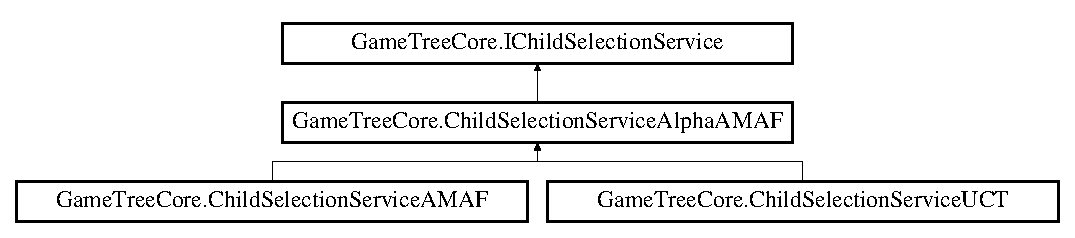
\includegraphics[height=2.754098cm]{class_game_tree_core_1_1_child_selection_service_alpha_a_m_a_f}
\end{center}
\end{figure}
\subsection*{Public Member Functions}
\begin{DoxyCompactItemize}
\item 
\mbox{\hyperlink{class_game_tree_core_1_1_child_selection_service_alpha_a_m_a_f_a0066b042bfcf03ce6f48bb0e2c2f686c}{Child\+Selection\+Service\+Alpha\+A\+M\+AF}} (double alpha)
\begin{DoxyCompactList}\small\item\em Creates a new instance of the \mbox{\hyperlink{class_game_tree_core_1_1_child_selection_service_alpha_a_m_a_f}{Child\+Selection\+Service\+Alpha\+A\+M\+AF}} class. \end{DoxyCompactList}\item 
override string \mbox{\hyperlink{class_game_tree_core_1_1_child_selection_service_alpha_a_m_a_f_a363afde50466810de65b08e58b96be8d}{To\+String}} ()
\begin{DoxyCompactList}\small\item\em Returns a string with informations about the child selection service. \end{DoxyCompactList}\item 
\mbox{\hyperlink{interface_game_tree_core_1_1_i_game_tree_node}{I\+Game\+Tree\+Node}} \mbox{\hyperlink{class_game_tree_core_1_1_child_selection_service_alpha_a_m_a_f_af0d4f97cb4f3ba63de5985c899f1ab3d}{child\+Selection}} (\mbox{\hyperlink{interface_game_tree_core_1_1_i_game_tree_node}{I\+Game\+Tree\+Node}} node, double exploration\+Constant)
\begin{DoxyCompactList}\small\item\em Selects the best child of the given node via the alpha A\+M\+AF algorithm. \end{DoxyCompactList}\end{DoxyCompactItemize}


\subsection{Detailed Description}
A child selection service based on the alpha A\+M\+AF algorithm. 



Definition at line 8 of file Child\+Selection\+Service\+Alpha\+A\+M\+A\+F.\+cs.



\subsection{Constructor \& Destructor Documentation}
\mbox{\Hypertarget{class_game_tree_core_1_1_child_selection_service_alpha_a_m_a_f_a0066b042bfcf03ce6f48bb0e2c2f686c}\label{class_game_tree_core_1_1_child_selection_service_alpha_a_m_a_f_a0066b042bfcf03ce6f48bb0e2c2f686c}} 
\index{Game\+Tree\+Core\+::\+Child\+Selection\+Service\+Alpha\+A\+M\+AF@{Game\+Tree\+Core\+::\+Child\+Selection\+Service\+Alpha\+A\+M\+AF}!Child\+Selection\+Service\+Alpha\+A\+M\+AF@{Child\+Selection\+Service\+Alpha\+A\+M\+AF}}
\index{Child\+Selection\+Service\+Alpha\+A\+M\+AF@{Child\+Selection\+Service\+Alpha\+A\+M\+AF}!Game\+Tree\+Core\+::\+Child\+Selection\+Service\+Alpha\+A\+M\+AF@{Game\+Tree\+Core\+::\+Child\+Selection\+Service\+Alpha\+A\+M\+AF}}
\subsubsection{\texorpdfstring{Child\+Selection\+Service\+Alpha\+A\+M\+A\+F()}{ChildSelectionServiceAlphaAMAF()}}
{\footnotesize\ttfamily Game\+Tree\+Core.\+Child\+Selection\+Service\+Alpha\+A\+M\+A\+F.\+Child\+Selection\+Service\+Alpha\+A\+M\+AF (\begin{DoxyParamCaption}\item[{double}]{alpha }\end{DoxyParamCaption})}



Creates a new instance of the \mbox{\hyperlink{class_game_tree_core_1_1_child_selection_service_alpha_a_m_a_f}{Child\+Selection\+Service\+Alpha\+A\+M\+AF}} class. 


\begin{DoxyParams}{Parameters}
{\em alpha} & A parameter in \mbox{[}0,1\mbox{]}.\\
\hline
\end{DoxyParams}

\begin{DoxyExceptions}{Exceptions}
{\em Argument\+Exception} & Is thrown if the given alpha is not in \mbox{[}0,1\mbox{]}.\\
\hline
\end{DoxyExceptions}


Definition at line 16 of file Child\+Selection\+Service\+Alpha\+A\+M\+A\+F.\+cs.



\subsection{Member Function Documentation}
\mbox{\Hypertarget{class_game_tree_core_1_1_child_selection_service_alpha_a_m_a_f_af0d4f97cb4f3ba63de5985c899f1ab3d}\label{class_game_tree_core_1_1_child_selection_service_alpha_a_m_a_f_af0d4f97cb4f3ba63de5985c899f1ab3d}} 
\index{Game\+Tree\+Core\+::\+Child\+Selection\+Service\+Alpha\+A\+M\+AF@{Game\+Tree\+Core\+::\+Child\+Selection\+Service\+Alpha\+A\+M\+AF}!child\+Selection@{child\+Selection}}
\index{child\+Selection@{child\+Selection}!Game\+Tree\+Core\+::\+Child\+Selection\+Service\+Alpha\+A\+M\+AF@{Game\+Tree\+Core\+::\+Child\+Selection\+Service\+Alpha\+A\+M\+AF}}
\subsubsection{\texorpdfstring{child\+Selection()}{childSelection()}}
{\footnotesize\ttfamily \mbox{\hyperlink{interface_game_tree_core_1_1_i_game_tree_node}{I\+Game\+Tree\+Node}} Game\+Tree\+Core.\+Child\+Selection\+Service\+Alpha\+A\+M\+A\+F.\+child\+Selection (\begin{DoxyParamCaption}\item[{\mbox{\hyperlink{interface_game_tree_core_1_1_i_game_tree_node}{I\+Game\+Tree\+Node}}}]{node,  }\item[{double}]{exploration\+Constant }\end{DoxyParamCaption})}



Selects the best child of the given node via the alpha A\+M\+AF algorithm. 


\begin{DoxyParams}{Parameters}
{\em node} & A node in the game tree.\\
\hline
{\em exploration\+Constant} & A tunable exploration constant.\\
\hline
\end{DoxyParams}

\begin{DoxyExceptions}{Exceptions}
{\em Argument\+Null\+Exception} & Is thrown, if the given node is null.\\
\hline
{\em Invalid\+Operation\+Exception} & Is thrown, if no child nodes are available.\\
\hline
\end{DoxyExceptions}


Implements \mbox{\hyperlink{interface_game_tree_core_1_1_i_child_selection_service}{Game\+Tree\+Core.\+I\+Child\+Selection\+Service}}.



Definition at line 36 of file Child\+Selection\+Service\+Alpha\+A\+M\+A\+F.\+cs.

\mbox{\Hypertarget{class_game_tree_core_1_1_child_selection_service_alpha_a_m_a_f_a363afde50466810de65b08e58b96be8d}\label{class_game_tree_core_1_1_child_selection_service_alpha_a_m_a_f_a363afde50466810de65b08e58b96be8d}} 
\index{Game\+Tree\+Core\+::\+Child\+Selection\+Service\+Alpha\+A\+M\+AF@{Game\+Tree\+Core\+::\+Child\+Selection\+Service\+Alpha\+A\+M\+AF}!To\+String@{To\+String}}
\index{To\+String@{To\+String}!Game\+Tree\+Core\+::\+Child\+Selection\+Service\+Alpha\+A\+M\+AF@{Game\+Tree\+Core\+::\+Child\+Selection\+Service\+Alpha\+A\+M\+AF}}
\subsubsection{\texorpdfstring{To\+String()}{ToString()}}
{\footnotesize\ttfamily override string Game\+Tree\+Core.\+Child\+Selection\+Service\+Alpha\+A\+M\+A\+F.\+To\+String (\begin{DoxyParamCaption}{ }\end{DoxyParamCaption})}



Returns a string with informations about the child selection service. 



Definition at line 25 of file Child\+Selection\+Service\+Alpha\+A\+M\+A\+F.\+cs.


\hypertarget{class_game_tree_core_1_1_child_selection_service_a_m_a_f}{}\section{Game\+Tree\+Core.\+Child\+Selection\+Service\+A\+M\+AF Class Reference}
\label{class_game_tree_core_1_1_child_selection_service_a_m_a_f}\index{Game\+Tree\+Core.\+Child\+Selection\+Service\+A\+M\+AF@{Game\+Tree\+Core.\+Child\+Selection\+Service\+A\+M\+AF}}


A child selection service based on the A\+M\+AF algorithm. This is a special case of the alpha A\+M\+AF version (alpha = 1).  


Inheritance diagram for Game\+Tree\+Core.\+Child\+Selection\+Service\+A\+M\+AF\+:\begin{figure}[H]
\begin{center}
\leavevmode
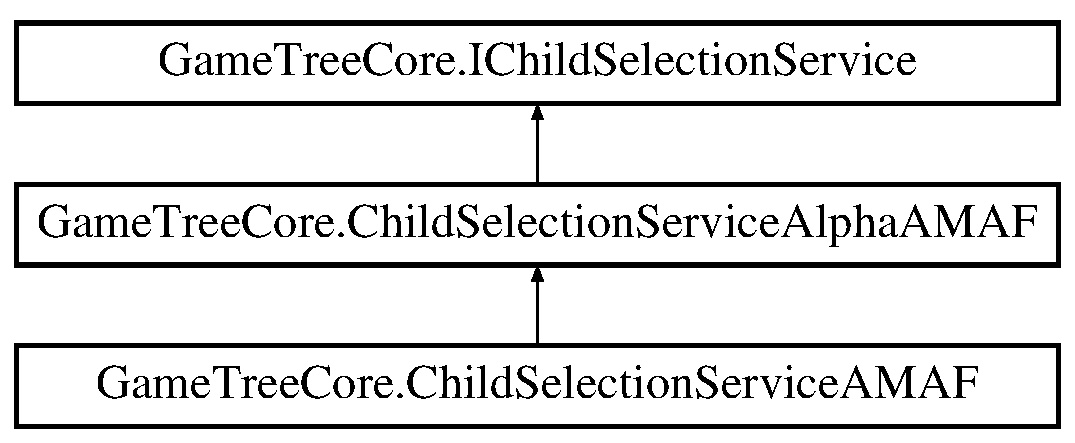
\includegraphics[height=3.000000cm]{class_game_tree_core_1_1_child_selection_service_a_m_a_f}
\end{center}
\end{figure}
\subsection*{Public Member Functions}
\begin{DoxyCompactItemize}
\item 
\mbox{\hyperlink{class_game_tree_core_1_1_child_selection_service_a_m_a_f_a3dfbd210da9fcf10fd87fdda9015f1b0}{Child\+Selection\+Service\+A\+M\+AF}} ()
\begin{DoxyCompactList}\small\item\em Creates a new instance of the \mbox{\hyperlink{class_game_tree_core_1_1_child_selection_service_a_m_a_f}{Child\+Selection\+Service\+A\+M\+AF}} class. \end{DoxyCompactList}\item 
override string \mbox{\hyperlink{class_game_tree_core_1_1_child_selection_service_a_m_a_f_aac59ed66cb99284d847efe69dbe62b22}{To\+String}} ()
\begin{DoxyCompactList}\small\item\em Returns a string with informations about the child selection service. \end{DoxyCompactList}\end{DoxyCompactItemize}


\subsection{Detailed Description}
A child selection service based on the A\+M\+AF algorithm. This is a special case of the alpha A\+M\+AF version (alpha = 1). 



Definition at line 5 of file Child\+Selection\+Service\+A\+M\+A\+F.\+cs.



\subsection{Constructor \& Destructor Documentation}
\mbox{\Hypertarget{class_game_tree_core_1_1_child_selection_service_a_m_a_f_a3dfbd210da9fcf10fd87fdda9015f1b0}\label{class_game_tree_core_1_1_child_selection_service_a_m_a_f_a3dfbd210da9fcf10fd87fdda9015f1b0}} 
\index{Game\+Tree\+Core\+::\+Child\+Selection\+Service\+A\+M\+AF@{Game\+Tree\+Core\+::\+Child\+Selection\+Service\+A\+M\+AF}!Child\+Selection\+Service\+A\+M\+AF@{Child\+Selection\+Service\+A\+M\+AF}}
\index{Child\+Selection\+Service\+A\+M\+AF@{Child\+Selection\+Service\+A\+M\+AF}!Game\+Tree\+Core\+::\+Child\+Selection\+Service\+A\+M\+AF@{Game\+Tree\+Core\+::\+Child\+Selection\+Service\+A\+M\+AF}}
\subsubsection{\texorpdfstring{Child\+Selection\+Service\+A\+M\+A\+F()}{ChildSelectionServiceAMAF()}}
{\footnotesize\ttfamily Game\+Tree\+Core.\+Child\+Selection\+Service\+A\+M\+A\+F.\+Child\+Selection\+Service\+A\+M\+AF (\begin{DoxyParamCaption}{ }\end{DoxyParamCaption})}



Creates a new instance of the \mbox{\hyperlink{class_game_tree_core_1_1_child_selection_service_a_m_a_f}{Child\+Selection\+Service\+A\+M\+AF}} class. 



Definition at line 9 of file Child\+Selection\+Service\+A\+M\+A\+F.\+cs.



\subsection{Member Function Documentation}
\mbox{\Hypertarget{class_game_tree_core_1_1_child_selection_service_a_m_a_f_aac59ed66cb99284d847efe69dbe62b22}\label{class_game_tree_core_1_1_child_selection_service_a_m_a_f_aac59ed66cb99284d847efe69dbe62b22}} 
\index{Game\+Tree\+Core\+::\+Child\+Selection\+Service\+A\+M\+AF@{Game\+Tree\+Core\+::\+Child\+Selection\+Service\+A\+M\+AF}!To\+String@{To\+String}}
\index{To\+String@{To\+String}!Game\+Tree\+Core\+::\+Child\+Selection\+Service\+A\+M\+AF@{Game\+Tree\+Core\+::\+Child\+Selection\+Service\+A\+M\+AF}}
\subsubsection{\texorpdfstring{To\+String()}{ToString()}}
{\footnotesize\ttfamily override string Game\+Tree\+Core.\+Child\+Selection\+Service\+A\+M\+A\+F.\+To\+String (\begin{DoxyParamCaption}{ }\end{DoxyParamCaption})}



Returns a string with informations about the child selection service. 



Definition at line 15 of file Child\+Selection\+Service\+A\+M\+A\+F.\+cs.


\hypertarget{class_game_tree_core_1_1_child_selection_service_r_a_v_e}{}\section{Game\+Tree\+Core.\+Child\+Selection\+Service\+R\+A\+VE Class Reference}
\label{class_game_tree_core_1_1_child_selection_service_r_a_v_e}\index{Game\+Tree\+Core.\+Child\+Selection\+Service\+R\+A\+VE@{Game\+Tree\+Core.\+Child\+Selection\+Service\+R\+A\+VE}}


A child selection service based on the R\+A\+VE algorithm.  


Inheritance diagram for Game\+Tree\+Core.\+Child\+Selection\+Service\+R\+A\+VE\+:\begin{figure}[H]
\begin{center}
\leavevmode
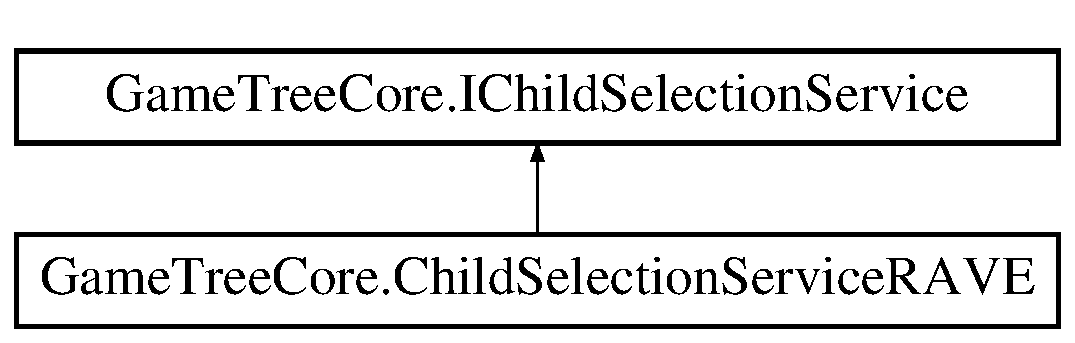
\includegraphics[height=2.000000cm]{class_game_tree_core_1_1_child_selection_service_r_a_v_e}
\end{center}
\end{figure}
\subsection*{Public Member Functions}
\begin{DoxyCompactItemize}
\item 
\mbox{\hyperlink{class_game_tree_core_1_1_child_selection_service_r_a_v_e_a45079106ea7e731b606699e6c5123c14}{Child\+Selection\+Service\+R\+A\+VE}} (int playouts\+Bound)
\begin{DoxyCompactList}\small\item\em Creates a new instance of the \mbox{\hyperlink{class_game_tree_core_1_1_child_selection_service_r_a_v_e}{Child\+Selection\+Service\+R\+A\+VE}} class. \end{DoxyCompactList}\item 
override string \mbox{\hyperlink{class_game_tree_core_1_1_child_selection_service_r_a_v_e_a995e1c2dfd72caa32cee278de8a836fc}{To\+String}} ()
\begin{DoxyCompactList}\small\item\em Returns a string with informations about the child selection service. \end{DoxyCompactList}\item 
\mbox{\hyperlink{interface_game_tree_core_1_1_i_game_tree_node}{I\+Game\+Tree\+Node}} \mbox{\hyperlink{class_game_tree_core_1_1_child_selection_service_r_a_v_e_a5a6fe93864c94224724eee96f51fd9af}{child\+Selection}} (\mbox{\hyperlink{interface_game_tree_core_1_1_i_game_tree_node}{I\+Game\+Tree\+Node}} node, double exploration\+Constant)
\begin{DoxyCompactList}\small\item\em Selects the best child of the given node via the R\+A\+VE algorithm. \end{DoxyCompactList}\end{DoxyCompactItemize}


\subsection{Detailed Description}
A child selection service based on the R\+A\+VE algorithm. 



Definition at line 8 of file Child\+Selection\+Service\+R\+A\+V\+E.\+cs.



\subsection{Constructor \& Destructor Documentation}
\mbox{\Hypertarget{class_game_tree_core_1_1_child_selection_service_r_a_v_e_a45079106ea7e731b606699e6c5123c14}\label{class_game_tree_core_1_1_child_selection_service_r_a_v_e_a45079106ea7e731b606699e6c5123c14}} 
\index{Game\+Tree\+Core\+::\+Child\+Selection\+Service\+R\+A\+VE@{Game\+Tree\+Core\+::\+Child\+Selection\+Service\+R\+A\+VE}!Child\+Selection\+Service\+R\+A\+VE@{Child\+Selection\+Service\+R\+A\+VE}}
\index{Child\+Selection\+Service\+R\+A\+VE@{Child\+Selection\+Service\+R\+A\+VE}!Game\+Tree\+Core\+::\+Child\+Selection\+Service\+R\+A\+VE@{Game\+Tree\+Core\+::\+Child\+Selection\+Service\+R\+A\+VE}}
\subsubsection{\texorpdfstring{Child\+Selection\+Service\+R\+A\+V\+E()}{ChildSelectionServiceRAVE()}}
{\footnotesize\ttfamily Game\+Tree\+Core.\+Child\+Selection\+Service\+R\+A\+V\+E.\+Child\+Selection\+Service\+R\+A\+VE (\begin{DoxyParamCaption}\item[{int}]{playouts\+Bound }\end{DoxyParamCaption})}



Creates a new instance of the \mbox{\hyperlink{class_game_tree_core_1_1_child_selection_service_r_a_v_e}{Child\+Selection\+Service\+R\+A\+VE}} class. 


\begin{DoxyParams}{Parameters}
{\em playouts\+Bound} & A nonzero playouts bound.\\
\hline
\end{DoxyParams}

\begin{DoxyExceptions}{Exceptions}
{\em Argument\+Exception} & Is thrown, if the given bound is negative.\\
\hline
\end{DoxyExceptions}


Definition at line 17 of file Child\+Selection\+Service\+R\+A\+V\+E.\+cs.



\subsection{Member Function Documentation}
\mbox{\Hypertarget{class_game_tree_core_1_1_child_selection_service_r_a_v_e_a5a6fe93864c94224724eee96f51fd9af}\label{class_game_tree_core_1_1_child_selection_service_r_a_v_e_a5a6fe93864c94224724eee96f51fd9af}} 
\index{Game\+Tree\+Core\+::\+Child\+Selection\+Service\+R\+A\+VE@{Game\+Tree\+Core\+::\+Child\+Selection\+Service\+R\+A\+VE}!child\+Selection@{child\+Selection}}
\index{child\+Selection@{child\+Selection}!Game\+Tree\+Core\+::\+Child\+Selection\+Service\+R\+A\+VE@{Game\+Tree\+Core\+::\+Child\+Selection\+Service\+R\+A\+VE}}
\subsubsection{\texorpdfstring{child\+Selection()}{childSelection()}}
{\footnotesize\ttfamily \mbox{\hyperlink{interface_game_tree_core_1_1_i_game_tree_node}{I\+Game\+Tree\+Node}} Game\+Tree\+Core.\+Child\+Selection\+Service\+R\+A\+V\+E.\+child\+Selection (\begin{DoxyParamCaption}\item[{\mbox{\hyperlink{interface_game_tree_core_1_1_i_game_tree_node}{I\+Game\+Tree\+Node}}}]{node,  }\item[{double}]{exploration\+Constant }\end{DoxyParamCaption})}



Selects the best child of the given node via the R\+A\+VE algorithm. 


\begin{DoxyParams}{Parameters}
{\em node} & A node in the game tree.\\
\hline
{\em exploration\+Constant} & A tunable exploration constant.\\
\hline
\end{DoxyParams}

\begin{DoxyExceptions}{Exceptions}
{\em Argument\+Null\+Exception} & Is thrown, if the given node is null.\\
\hline
{\em Invalid\+Operation\+Exception} & Is thrown, if no child nodes are available.\\
\hline
\end{DoxyExceptions}


Implements \mbox{\hyperlink{interface_game_tree_core_1_1_i_child_selection_service}{Game\+Tree\+Core.\+I\+Child\+Selection\+Service}}.



Definition at line 37 of file Child\+Selection\+Service\+R\+A\+V\+E.\+cs.

\mbox{\Hypertarget{class_game_tree_core_1_1_child_selection_service_r_a_v_e_a995e1c2dfd72caa32cee278de8a836fc}\label{class_game_tree_core_1_1_child_selection_service_r_a_v_e_a995e1c2dfd72caa32cee278de8a836fc}} 
\index{Game\+Tree\+Core\+::\+Child\+Selection\+Service\+R\+A\+VE@{Game\+Tree\+Core\+::\+Child\+Selection\+Service\+R\+A\+VE}!To\+String@{To\+String}}
\index{To\+String@{To\+String}!Game\+Tree\+Core\+::\+Child\+Selection\+Service\+R\+A\+VE@{Game\+Tree\+Core\+::\+Child\+Selection\+Service\+R\+A\+VE}}
\subsubsection{\texorpdfstring{To\+String()}{ToString()}}
{\footnotesize\ttfamily override string Game\+Tree\+Core.\+Child\+Selection\+Service\+R\+A\+V\+E.\+To\+String (\begin{DoxyParamCaption}{ }\end{DoxyParamCaption})}



Returns a string with informations about the child selection service. 



Definition at line 26 of file Child\+Selection\+Service\+R\+A\+V\+E.\+cs.


\hypertarget{class_game_tree_core_1_1_child_selection_service_silver_alpha_a_m_a_f}{}\section{Game\+Tree\+Core.\+Child\+Selection\+Service\+Silver\+Alpha\+A\+M\+AF Class Reference}
\label{class_game_tree_core_1_1_child_selection_service_silver_alpha_a_m_a_f}\index{Game\+Tree\+Core.\+Child\+Selection\+Service\+Silver\+Alpha\+A\+M\+AF@{Game\+Tree\+Core.\+Child\+Selection\+Service\+Silver\+Alpha\+A\+M\+AF}}


A child selection service based on the alpha A\+M\+AF algorithm from David Silver.  


Inheritance diagram for Game\+Tree\+Core.\+Child\+Selection\+Service\+Silver\+Alpha\+A\+M\+AF\+:\begin{figure}[H]
\begin{center}
\leavevmode
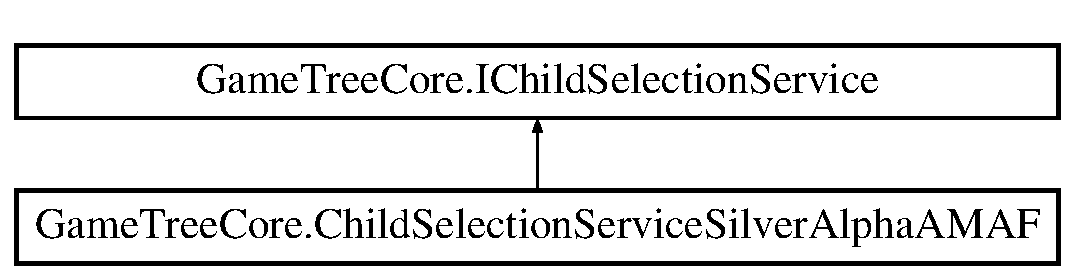
\includegraphics[height=2.000000cm]{class_game_tree_core_1_1_child_selection_service_silver_alpha_a_m_a_f}
\end{center}
\end{figure}
\subsection*{Public Member Functions}
\begin{DoxyCompactItemize}
\item 
\mbox{\hyperlink{class_game_tree_core_1_1_child_selection_service_silver_alpha_a_m_a_f_a9f0b3952f37fab8b91e69950263934a7}{Child\+Selection\+Service\+Silver\+Alpha\+A\+M\+AF}} (double bias)
\begin{DoxyCompactList}\small\item\em Creates a new instance of the \mbox{\hyperlink{class_game_tree_core_1_1_child_selection_service_silver_alpha_a_m_a_f}{Child\+Selection\+Service\+Silver\+Alpha\+A\+M\+AF}} class. \end{DoxyCompactList}\item 
override string \mbox{\hyperlink{class_game_tree_core_1_1_child_selection_service_silver_alpha_a_m_a_f_a205abab62a400c3aa5bf9830047249dd}{To\+String}} ()
\begin{DoxyCompactList}\small\item\em Returns a string with informations about the child selection service. \end{DoxyCompactList}\item 
\mbox{\hyperlink{interface_game_tree_core_1_1_i_game_tree_node}{I\+Game\+Tree\+Node}} \mbox{\hyperlink{class_game_tree_core_1_1_child_selection_service_silver_alpha_a_m_a_f_af06bf48345ee92a0057b6cc9dbd47a9e}{child\+Selection}} (\mbox{\hyperlink{interface_game_tree_core_1_1_i_game_tree_node}{I\+Game\+Tree\+Node}} node, double exploration\+Constant)
\begin{DoxyCompactList}\small\item\em Selects the best child of the given node via the alpha A\+M\+AF algorithm from Silver. \end{DoxyCompactList}\end{DoxyCompactItemize}


\subsection{Detailed Description}
A child selection service based on the alpha A\+M\+AF algorithm from David Silver. 



Definition at line 8 of file Child\+Selection\+Service\+Silver\+Alpha\+A\+M\+A\+F.\+cs.



\subsection{Constructor \& Destructor Documentation}
\mbox{\Hypertarget{class_game_tree_core_1_1_child_selection_service_silver_alpha_a_m_a_f_a9f0b3952f37fab8b91e69950263934a7}\label{class_game_tree_core_1_1_child_selection_service_silver_alpha_a_m_a_f_a9f0b3952f37fab8b91e69950263934a7}} 
\index{Game\+Tree\+Core\+::\+Child\+Selection\+Service\+Silver\+Alpha\+A\+M\+AF@{Game\+Tree\+Core\+::\+Child\+Selection\+Service\+Silver\+Alpha\+A\+M\+AF}!Child\+Selection\+Service\+Silver\+Alpha\+A\+M\+AF@{Child\+Selection\+Service\+Silver\+Alpha\+A\+M\+AF}}
\index{Child\+Selection\+Service\+Silver\+Alpha\+A\+M\+AF@{Child\+Selection\+Service\+Silver\+Alpha\+A\+M\+AF}!Game\+Tree\+Core\+::\+Child\+Selection\+Service\+Silver\+Alpha\+A\+M\+AF@{Game\+Tree\+Core\+::\+Child\+Selection\+Service\+Silver\+Alpha\+A\+M\+AF}}
\subsubsection{\texorpdfstring{Child\+Selection\+Service\+Silver\+Alpha\+A\+M\+A\+F()}{ChildSelectionServiceSilverAlphaAMAF()}}
{\footnotesize\ttfamily Game\+Tree\+Core.\+Child\+Selection\+Service\+Silver\+Alpha\+A\+M\+A\+F.\+Child\+Selection\+Service\+Silver\+Alpha\+A\+M\+AF (\begin{DoxyParamCaption}\item[{double}]{bias }\end{DoxyParamCaption})}



Creates a new instance of the \mbox{\hyperlink{class_game_tree_core_1_1_child_selection_service_silver_alpha_a_m_a_f}{Child\+Selection\+Service\+Silver\+Alpha\+A\+M\+AF}} class. 


\begin{DoxyParams}{Parameters}
{\em bias} & A bias.\\
\hline
\end{DoxyParams}


Definition at line 16 of file Child\+Selection\+Service\+Silver\+Alpha\+A\+M\+A\+F.\+cs.



\subsection{Member Function Documentation}
\mbox{\Hypertarget{class_game_tree_core_1_1_child_selection_service_silver_alpha_a_m_a_f_af06bf48345ee92a0057b6cc9dbd47a9e}\label{class_game_tree_core_1_1_child_selection_service_silver_alpha_a_m_a_f_af06bf48345ee92a0057b6cc9dbd47a9e}} 
\index{Game\+Tree\+Core\+::\+Child\+Selection\+Service\+Silver\+Alpha\+A\+M\+AF@{Game\+Tree\+Core\+::\+Child\+Selection\+Service\+Silver\+Alpha\+A\+M\+AF}!child\+Selection@{child\+Selection}}
\index{child\+Selection@{child\+Selection}!Game\+Tree\+Core\+::\+Child\+Selection\+Service\+Silver\+Alpha\+A\+M\+AF@{Game\+Tree\+Core\+::\+Child\+Selection\+Service\+Silver\+Alpha\+A\+M\+AF}}
\subsubsection{\texorpdfstring{child\+Selection()}{childSelection()}}
{\footnotesize\ttfamily \mbox{\hyperlink{interface_game_tree_core_1_1_i_game_tree_node}{I\+Game\+Tree\+Node}} Game\+Tree\+Core.\+Child\+Selection\+Service\+Silver\+Alpha\+A\+M\+A\+F.\+child\+Selection (\begin{DoxyParamCaption}\item[{\mbox{\hyperlink{interface_game_tree_core_1_1_i_game_tree_node}{I\+Game\+Tree\+Node}}}]{node,  }\item[{double}]{exploration\+Constant }\end{DoxyParamCaption})}



Selects the best child of the given node via the alpha A\+M\+AF algorithm from Silver. 


\begin{DoxyParams}{Parameters}
{\em node} & A node in the game tree.\\
\hline
{\em exploration\+Constant} & A tunable exploration constant.\\
\hline
\end{DoxyParams}

\begin{DoxyExceptions}{Exceptions}
{\em Argument\+Null\+Exception} & Is thrown, if the given node is null.\\
\hline
{\em Invalid\+Operation\+Exception} & Is thrown, if no child nodes are available.\\
\hline
\end{DoxyExceptions}


Implements \mbox{\hyperlink{interface_game_tree_core_1_1_i_child_selection_service}{Game\+Tree\+Core.\+I\+Child\+Selection\+Service}}.



Definition at line 34 of file Child\+Selection\+Service\+Silver\+Alpha\+A\+M\+A\+F.\+cs.

\mbox{\Hypertarget{class_game_tree_core_1_1_child_selection_service_silver_alpha_a_m_a_f_a205abab62a400c3aa5bf9830047249dd}\label{class_game_tree_core_1_1_child_selection_service_silver_alpha_a_m_a_f_a205abab62a400c3aa5bf9830047249dd}} 
\index{Game\+Tree\+Core\+::\+Child\+Selection\+Service\+Silver\+Alpha\+A\+M\+AF@{Game\+Tree\+Core\+::\+Child\+Selection\+Service\+Silver\+Alpha\+A\+M\+AF}!To\+String@{To\+String}}
\index{To\+String@{To\+String}!Game\+Tree\+Core\+::\+Child\+Selection\+Service\+Silver\+Alpha\+A\+M\+AF@{Game\+Tree\+Core\+::\+Child\+Selection\+Service\+Silver\+Alpha\+A\+M\+AF}}
\subsubsection{\texorpdfstring{To\+String()}{ToString()}}
{\footnotesize\ttfamily override string Game\+Tree\+Core.\+Child\+Selection\+Service\+Silver\+Alpha\+A\+M\+A\+F.\+To\+String (\begin{DoxyParamCaption}{ }\end{DoxyParamCaption})}



Returns a string with informations about the child selection service. 



Definition at line 23 of file Child\+Selection\+Service\+Silver\+Alpha\+A\+M\+A\+F.\+cs.


\hypertarget{class_game_tree_core_1_1_child_selection_service_u_c_t}{}\section{Game\+Tree\+Core.\+Child\+Selection\+Service\+U\+CT Class Reference}
\label{class_game_tree_core_1_1_child_selection_service_u_c_t}\index{Game\+Tree\+Core.\+Child\+Selection\+Service\+U\+CT@{Game\+Tree\+Core.\+Child\+Selection\+Service\+U\+CT}}


A child selection service based on the U\+CT algorithm. This is a special case of the alpha A\+M\+AF version (alpha = 0).  


Inheritance diagram for Game\+Tree\+Core.\+Child\+Selection\+Service\+U\+CT\+:\begin{figure}[H]
\begin{center}
\leavevmode
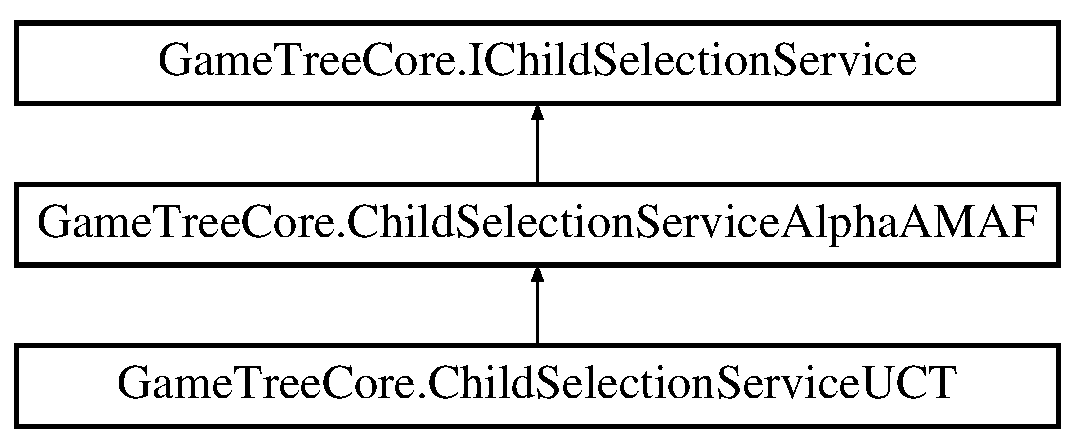
\includegraphics[height=3.000000cm]{class_game_tree_core_1_1_child_selection_service_u_c_t}
\end{center}
\end{figure}
\subsection*{Public Member Functions}
\begin{DoxyCompactItemize}
\item 
\mbox{\hyperlink{class_game_tree_core_1_1_child_selection_service_u_c_t_ad649e695f196bc3e4c3899aa591a9aee}{Child\+Selection\+Service\+U\+CT}} ()
\begin{DoxyCompactList}\small\item\em Creates a new instance of the \mbox{\hyperlink{class_game_tree_core_1_1_child_selection_service_u_c_t}{Child\+Selection\+Service\+U\+CT}} class. \end{DoxyCompactList}\item 
override string \mbox{\hyperlink{class_game_tree_core_1_1_child_selection_service_u_c_t_abbd068c35c9e9b2fd596b80a16c660fa}{To\+String}} ()
\begin{DoxyCompactList}\small\item\em Returns a string with informations about the child selection service. \end{DoxyCompactList}\end{DoxyCompactItemize}


\subsection{Detailed Description}
A child selection service based on the U\+CT algorithm. This is a special case of the alpha A\+M\+AF version (alpha = 0). 



Definition at line 5 of file Child\+Selection\+Service\+U\+C\+T.\+cs.



\subsection{Constructor \& Destructor Documentation}
\mbox{\Hypertarget{class_game_tree_core_1_1_child_selection_service_u_c_t_ad649e695f196bc3e4c3899aa591a9aee}\label{class_game_tree_core_1_1_child_selection_service_u_c_t_ad649e695f196bc3e4c3899aa591a9aee}} 
\index{Game\+Tree\+Core\+::\+Child\+Selection\+Service\+U\+CT@{Game\+Tree\+Core\+::\+Child\+Selection\+Service\+U\+CT}!Child\+Selection\+Service\+U\+CT@{Child\+Selection\+Service\+U\+CT}}
\index{Child\+Selection\+Service\+U\+CT@{Child\+Selection\+Service\+U\+CT}!Game\+Tree\+Core\+::\+Child\+Selection\+Service\+U\+CT@{Game\+Tree\+Core\+::\+Child\+Selection\+Service\+U\+CT}}
\subsubsection{\texorpdfstring{Child\+Selection\+Service\+U\+C\+T()}{ChildSelectionServiceUCT()}}
{\footnotesize\ttfamily Game\+Tree\+Core.\+Child\+Selection\+Service\+U\+C\+T.\+Child\+Selection\+Service\+U\+CT (\begin{DoxyParamCaption}{ }\end{DoxyParamCaption})}



Creates a new instance of the \mbox{\hyperlink{class_game_tree_core_1_1_child_selection_service_u_c_t}{Child\+Selection\+Service\+U\+CT}} class. 



Definition at line 9 of file Child\+Selection\+Service\+U\+C\+T.\+cs.



\subsection{Member Function Documentation}
\mbox{\Hypertarget{class_game_tree_core_1_1_child_selection_service_u_c_t_abbd068c35c9e9b2fd596b80a16c660fa}\label{class_game_tree_core_1_1_child_selection_service_u_c_t_abbd068c35c9e9b2fd596b80a16c660fa}} 
\index{Game\+Tree\+Core\+::\+Child\+Selection\+Service\+U\+CT@{Game\+Tree\+Core\+::\+Child\+Selection\+Service\+U\+CT}!To\+String@{To\+String}}
\index{To\+String@{To\+String}!Game\+Tree\+Core\+::\+Child\+Selection\+Service\+U\+CT@{Game\+Tree\+Core\+::\+Child\+Selection\+Service\+U\+CT}}
\subsubsection{\texorpdfstring{To\+String()}{ToString()}}
{\footnotesize\ttfamily override string Game\+Tree\+Core.\+Child\+Selection\+Service\+U\+C\+T.\+To\+String (\begin{DoxyParamCaption}{ }\end{DoxyParamCaption})}



Returns a string with informations about the child selection service. 



Definition at line 15 of file Child\+Selection\+Service\+U\+C\+T.\+cs.


\hypertarget{class_game_tree_core_1_1_final_child_selection_service_m_a_x}{}\section{Game\+Tree\+Core.\+Final\+Child\+Selection\+Service\+M\+AX Class Reference}
\label{class_game_tree_core_1_1_final_child_selection_service_m_a_x}\index{Game\+Tree\+Core.\+Final\+Child\+Selection\+Service\+M\+AX@{Game\+Tree\+Core.\+Final\+Child\+Selection\+Service\+M\+AX}}
Inheritance diagram for Game\+Tree\+Core.\+Final\+Child\+Selection\+Service\+M\+AX\+:\begin{figure}[H]
\begin{center}
\leavevmode
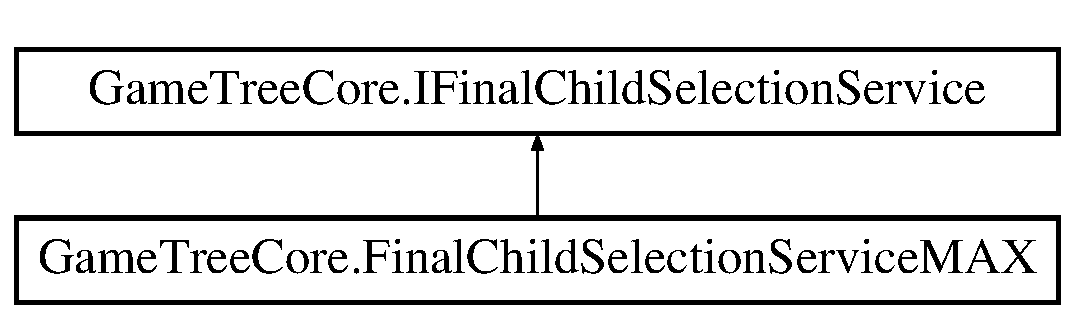
\includegraphics[height=2.000000cm]{class_game_tree_core_1_1_final_child_selection_service_m_a_x}
\end{center}
\end{figure}
\subsection*{Public Member Functions}
\begin{DoxyCompactItemize}
\item 
override string \mbox{\hyperlink{class_game_tree_core_1_1_final_child_selection_service_m_a_x_a56819f278cda4cf3a9b778cf53cca5c7}{To\+String}} ()
\begin{DoxyCompactList}\small\item\em Returns a string with informations about the child selection service. \end{DoxyCompactList}\item 
\mbox{\hyperlink{interface_game_tree_core_1_1_i_game_tree_node}{I\+Game\+Tree\+Node}} \mbox{\hyperlink{class_game_tree_core_1_1_final_child_selection_service_m_a_x_a15781c79f5979e4e60968463dd112fe4}{final\+Child\+Selection}} (\mbox{\hyperlink{interface_game_tree_core_1_1_i_game_tree_node}{I\+Game\+Tree\+Node}} node)
\begin{DoxyCompactList}\small\item\em Selects the child with the highest relative reward. \end{DoxyCompactList}\end{DoxyCompactItemize}


\subsection{Detailed Description}


Definition at line 5 of file Final\+Child\+Selection\+Service\+M\+A\+X.\+cs.



\subsection{Member Function Documentation}
\mbox{\Hypertarget{class_game_tree_core_1_1_final_child_selection_service_m_a_x_a15781c79f5979e4e60968463dd112fe4}\label{class_game_tree_core_1_1_final_child_selection_service_m_a_x_a15781c79f5979e4e60968463dd112fe4}} 
\index{Game\+Tree\+Core\+::\+Final\+Child\+Selection\+Service\+M\+AX@{Game\+Tree\+Core\+::\+Final\+Child\+Selection\+Service\+M\+AX}!final\+Child\+Selection@{final\+Child\+Selection}}
\index{final\+Child\+Selection@{final\+Child\+Selection}!Game\+Tree\+Core\+::\+Final\+Child\+Selection\+Service\+M\+AX@{Game\+Tree\+Core\+::\+Final\+Child\+Selection\+Service\+M\+AX}}
\subsubsection{\texorpdfstring{final\+Child\+Selection()}{finalChildSelection()}}
{\footnotesize\ttfamily \mbox{\hyperlink{interface_game_tree_core_1_1_i_game_tree_node}{I\+Game\+Tree\+Node}} Game\+Tree\+Core.\+Final\+Child\+Selection\+Service\+M\+A\+X.\+final\+Child\+Selection (\begin{DoxyParamCaption}\item[{\mbox{\hyperlink{interface_game_tree_core_1_1_i_game_tree_node}{I\+Game\+Tree\+Node}}}]{node }\end{DoxyParamCaption})}



Selects the child with the highest relative reward. 


\begin{DoxyParams}{Parameters}
{\em node} & A node.\\
\hline
\end{DoxyParams}

\begin{DoxyExceptions}{Exceptions}
{\em Argument\+Null\+Exception} & Is thrown, if the given node is null.\\
\hline
{\em Invalid\+Operation\+Exception} & Is thrown, if no child nodes are available.\\
\hline
\end{DoxyExceptions}


Implements \mbox{\hyperlink{interface_game_tree_core_1_1_i_final_child_selection_service}{Game\+Tree\+Core.\+I\+Final\+Child\+Selection\+Service}}.



Definition at line 19 of file Final\+Child\+Selection\+Service\+M\+A\+X.\+cs.

\mbox{\Hypertarget{class_game_tree_core_1_1_final_child_selection_service_m_a_x_a56819f278cda4cf3a9b778cf53cca5c7}\label{class_game_tree_core_1_1_final_child_selection_service_m_a_x_a56819f278cda4cf3a9b778cf53cca5c7}} 
\index{Game\+Tree\+Core\+::\+Final\+Child\+Selection\+Service\+M\+AX@{Game\+Tree\+Core\+::\+Final\+Child\+Selection\+Service\+M\+AX}!To\+String@{To\+String}}
\index{To\+String@{To\+String}!Game\+Tree\+Core\+::\+Final\+Child\+Selection\+Service\+M\+AX@{Game\+Tree\+Core\+::\+Final\+Child\+Selection\+Service\+M\+AX}}
\subsubsection{\texorpdfstring{To\+String()}{ToString()}}
{\footnotesize\ttfamily override string Game\+Tree\+Core.\+Final\+Child\+Selection\+Service\+M\+A\+X.\+To\+String (\begin{DoxyParamCaption}{ }\end{DoxyParamCaption})}



Returns a string with informations about the child selection service. 



Definition at line 9 of file Final\+Child\+Selection\+Service\+M\+A\+X.\+cs.


\hypertarget{class_game_tree_core_1_1_final_child_selection_service_r_o_b_u_s_t}{}\section{Game\+Tree\+Core.\+Final\+Child\+Selection\+Service\+R\+O\+B\+U\+ST Class Reference}
\label{class_game_tree_core_1_1_final_child_selection_service_r_o_b_u_s_t}\index{Game\+Tree\+Core.\+Final\+Child\+Selection\+Service\+R\+O\+B\+U\+ST@{Game\+Tree\+Core.\+Final\+Child\+Selection\+Service\+R\+O\+B\+U\+ST}}
Inheritance diagram for Game\+Tree\+Core.\+Final\+Child\+Selection\+Service\+R\+O\+B\+U\+ST\+:\begin{figure}[H]
\begin{center}
\leavevmode
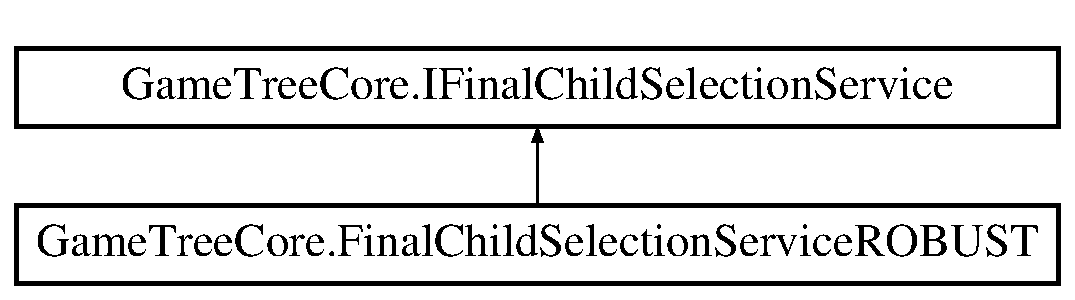
\includegraphics[height=2.000000cm]{class_game_tree_core_1_1_final_child_selection_service_r_o_b_u_s_t}
\end{center}
\end{figure}
\subsection*{Public Member Functions}
\begin{DoxyCompactItemize}
\item 
override string \mbox{\hyperlink{class_game_tree_core_1_1_final_child_selection_service_r_o_b_u_s_t_abf32995059eff3ba39b40d3dfa1ed512}{To\+String}} ()
\begin{DoxyCompactList}\small\item\em Returns a string with informations about the child selection service. \end{DoxyCompactList}\item 
\mbox{\hyperlink{interface_game_tree_core_1_1_i_game_tree_node}{I\+Game\+Tree\+Node}} \mbox{\hyperlink{class_game_tree_core_1_1_final_child_selection_service_r_o_b_u_s_t_a8863618ea3c7a12f1dee3774ab62888e}{final\+Child\+Selection}} (\mbox{\hyperlink{interface_game_tree_core_1_1_i_game_tree_node}{I\+Game\+Tree\+Node}} node)
\begin{DoxyCompactList}\small\item\em Selects the root child with the highest relative reward. \end{DoxyCompactList}\end{DoxyCompactItemize}


\subsection{Detailed Description}


Definition at line 5 of file Final\+Child\+Selection\+Service\+R\+O\+B\+U\+S\+T.\+cs.



\subsection{Member Function Documentation}
\mbox{\Hypertarget{class_game_tree_core_1_1_final_child_selection_service_r_o_b_u_s_t_a8863618ea3c7a12f1dee3774ab62888e}\label{class_game_tree_core_1_1_final_child_selection_service_r_o_b_u_s_t_a8863618ea3c7a12f1dee3774ab62888e}} 
\index{Game\+Tree\+Core\+::\+Final\+Child\+Selection\+Service\+R\+O\+B\+U\+ST@{Game\+Tree\+Core\+::\+Final\+Child\+Selection\+Service\+R\+O\+B\+U\+ST}!final\+Child\+Selection@{final\+Child\+Selection}}
\index{final\+Child\+Selection@{final\+Child\+Selection}!Game\+Tree\+Core\+::\+Final\+Child\+Selection\+Service\+R\+O\+B\+U\+ST@{Game\+Tree\+Core\+::\+Final\+Child\+Selection\+Service\+R\+O\+B\+U\+ST}}
\subsubsection{\texorpdfstring{final\+Child\+Selection()}{finalChildSelection()}}
{\footnotesize\ttfamily \mbox{\hyperlink{interface_game_tree_core_1_1_i_game_tree_node}{I\+Game\+Tree\+Node}} Game\+Tree\+Core.\+Final\+Child\+Selection\+Service\+R\+O\+B\+U\+S\+T.\+final\+Child\+Selection (\begin{DoxyParamCaption}\item[{\mbox{\hyperlink{interface_game_tree_core_1_1_i_game_tree_node}{I\+Game\+Tree\+Node}}}]{node }\end{DoxyParamCaption})}



Selects the root child with the highest relative reward. 


\begin{DoxyParams}{Parameters}
{\em node} & A node.\\
\hline
\end{DoxyParams}

\begin{DoxyExceptions}{Exceptions}
{\em Argument\+Null\+Exception} & Is thrown, if the given node is null.\\
\hline
{\em Invalid\+Operation\+Exception} & Is thrown, if no child nodes are available.\\
\hline
\end{DoxyExceptions}


Implements \mbox{\hyperlink{interface_game_tree_core_1_1_i_final_child_selection_service}{Game\+Tree\+Core.\+I\+Final\+Child\+Selection\+Service}}.



Definition at line 19 of file Final\+Child\+Selection\+Service\+R\+O\+B\+U\+S\+T.\+cs.

\mbox{\Hypertarget{class_game_tree_core_1_1_final_child_selection_service_r_o_b_u_s_t_abf32995059eff3ba39b40d3dfa1ed512}\label{class_game_tree_core_1_1_final_child_selection_service_r_o_b_u_s_t_abf32995059eff3ba39b40d3dfa1ed512}} 
\index{Game\+Tree\+Core\+::\+Final\+Child\+Selection\+Service\+R\+O\+B\+U\+ST@{Game\+Tree\+Core\+::\+Final\+Child\+Selection\+Service\+R\+O\+B\+U\+ST}!To\+String@{To\+String}}
\index{To\+String@{To\+String}!Game\+Tree\+Core\+::\+Final\+Child\+Selection\+Service\+R\+O\+B\+U\+ST@{Game\+Tree\+Core\+::\+Final\+Child\+Selection\+Service\+R\+O\+B\+U\+ST}}
\subsubsection{\texorpdfstring{To\+String()}{ToString()}}
{\footnotesize\ttfamily override string Game\+Tree\+Core.\+Final\+Child\+Selection\+Service\+R\+O\+B\+U\+S\+T.\+To\+String (\begin{DoxyParamCaption}{ }\end{DoxyParamCaption})}



Returns a string with informations about the child selection service. 



Definition at line 9 of file Final\+Child\+Selection\+Service\+R\+O\+B\+U\+S\+T.\+cs.


\hypertarget{class_game_tree_core_1_1_final_child_selection_service_s_e_c_u_r_e}{}\section{Game\+Tree\+Core.\+Final\+Child\+Selection\+Service\+S\+E\+C\+U\+RE Class Reference}
\label{class_game_tree_core_1_1_final_child_selection_service_s_e_c_u_r_e}\index{Game\+Tree\+Core.\+Final\+Child\+Selection\+Service\+S\+E\+C\+U\+RE@{Game\+Tree\+Core.\+Final\+Child\+Selection\+Service\+S\+E\+C\+U\+RE}}
Inheritance diagram for Game\+Tree\+Core.\+Final\+Child\+Selection\+Service\+S\+E\+C\+U\+RE\+:\begin{figure}[H]
\begin{center}
\leavevmode
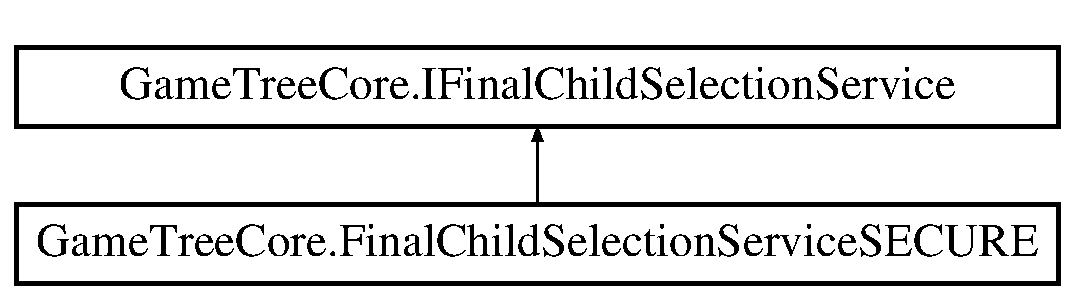
\includegraphics[height=2.000000cm]{class_game_tree_core_1_1_final_child_selection_service_s_e_c_u_r_e}
\end{center}
\end{figure}
\subsection*{Public Member Functions}
\begin{DoxyCompactItemize}
\item 
override string \mbox{\hyperlink{class_game_tree_core_1_1_final_child_selection_service_s_e_c_u_r_e_a4286392c639860e2f188f853b43f8103}{To\+String}} ()
\begin{DoxyCompactList}\small\item\em Returns a string with informations about the child selection service. \end{DoxyCompactList}\item 
\mbox{\hyperlink{interface_game_tree_core_1_1_i_game_tree_node}{I\+Game\+Tree\+Node}} \mbox{\hyperlink{class_game_tree_core_1_1_final_child_selection_service_s_e_c_u_r_e_a766a9bcee0b76d7f12e3093dc315bcc6}{final\+Child\+Selection}} (\mbox{\hyperlink{interface_game_tree_core_1_1_i_game_tree_node}{I\+Game\+Tree\+Node}} node)
\begin{DoxyCompactList}\small\item\em Selects the root child with the highest relative reward. \end{DoxyCompactList}\end{DoxyCompactItemize}


\subsection{Detailed Description}


Definition at line 5 of file Final\+Child\+Selection\+Service\+S\+E\+C\+U\+R\+E.\+cs.



\subsection{Member Function Documentation}
\mbox{\Hypertarget{class_game_tree_core_1_1_final_child_selection_service_s_e_c_u_r_e_a766a9bcee0b76d7f12e3093dc315bcc6}\label{class_game_tree_core_1_1_final_child_selection_service_s_e_c_u_r_e_a766a9bcee0b76d7f12e3093dc315bcc6}} 
\index{Game\+Tree\+Core\+::\+Final\+Child\+Selection\+Service\+S\+E\+C\+U\+RE@{Game\+Tree\+Core\+::\+Final\+Child\+Selection\+Service\+S\+E\+C\+U\+RE}!final\+Child\+Selection@{final\+Child\+Selection}}
\index{final\+Child\+Selection@{final\+Child\+Selection}!Game\+Tree\+Core\+::\+Final\+Child\+Selection\+Service\+S\+E\+C\+U\+RE@{Game\+Tree\+Core\+::\+Final\+Child\+Selection\+Service\+S\+E\+C\+U\+RE}}
\subsubsection{\texorpdfstring{final\+Child\+Selection()}{finalChildSelection()}}
{\footnotesize\ttfamily \mbox{\hyperlink{interface_game_tree_core_1_1_i_game_tree_node}{I\+Game\+Tree\+Node}} Game\+Tree\+Core.\+Final\+Child\+Selection\+Service\+S\+E\+C\+U\+R\+E.\+final\+Child\+Selection (\begin{DoxyParamCaption}\item[{\mbox{\hyperlink{interface_game_tree_core_1_1_i_game_tree_node}{I\+Game\+Tree\+Node}}}]{node }\end{DoxyParamCaption})}



Selects the root child with the highest relative reward. 


\begin{DoxyParams}{Parameters}
{\em node} & A node.\\
\hline
\end{DoxyParams}
\begin{DoxyReturn}{Returns}
The root child with the highest relative reward.
\end{DoxyReturn}

\begin{DoxyExceptions}{Exceptions}
{\em Argument\+Null\+Exception} & Is thrown, if the given node is null.\\
\hline
{\em Invalid\+Operation\+Exception} & Is thrown, if no child nodes are available.\\
\hline
\end{DoxyExceptions}


Implements \mbox{\hyperlink{interface_game_tree_core_1_1_i_final_child_selection_service}{Game\+Tree\+Core.\+I\+Final\+Child\+Selection\+Service}}.



Definition at line 20 of file Final\+Child\+Selection\+Service\+S\+E\+C\+U\+R\+E.\+cs.

\mbox{\Hypertarget{class_game_tree_core_1_1_final_child_selection_service_s_e_c_u_r_e_a4286392c639860e2f188f853b43f8103}\label{class_game_tree_core_1_1_final_child_selection_service_s_e_c_u_r_e_a4286392c639860e2f188f853b43f8103}} 
\index{Game\+Tree\+Core\+::\+Final\+Child\+Selection\+Service\+S\+E\+C\+U\+RE@{Game\+Tree\+Core\+::\+Final\+Child\+Selection\+Service\+S\+E\+C\+U\+RE}!To\+String@{To\+String}}
\index{To\+String@{To\+String}!Game\+Tree\+Core\+::\+Final\+Child\+Selection\+Service\+S\+E\+C\+U\+RE@{Game\+Tree\+Core\+::\+Final\+Child\+Selection\+Service\+S\+E\+C\+U\+RE}}
\subsubsection{\texorpdfstring{To\+String()}{ToString()}}
{\footnotesize\ttfamily override string Game\+Tree\+Core.\+Final\+Child\+Selection\+Service\+S\+E\+C\+U\+R\+E.\+To\+String (\begin{DoxyParamCaption}{ }\end{DoxyParamCaption})}



Returns a string with informations about the child selection service. 



Definition at line 9 of file Final\+Child\+Selection\+Service\+S\+E\+C\+U\+R\+E.\+cs.


\hypertarget{interface_game_tree_core_1_1_i_child_selection_service}{}\section{Game\+Tree\+Core.\+I\+Child\+Selection\+Service Interface Reference}
\label{interface_game_tree_core_1_1_i_child_selection_service}\index{Game\+Tree\+Core.\+I\+Child\+Selection\+Service@{Game\+Tree\+Core.\+I\+Child\+Selection\+Service}}


Exposes a method to select a child node from a \mbox{\hyperlink{interface_game_tree_core_1_1_i_game_tree_node}{I\+Game\+Tree\+Node}}.  


Inheritance diagram for Game\+Tree\+Core.\+I\+Child\+Selection\+Service\+:\begin{figure}[H]
\begin{center}
\leavevmode
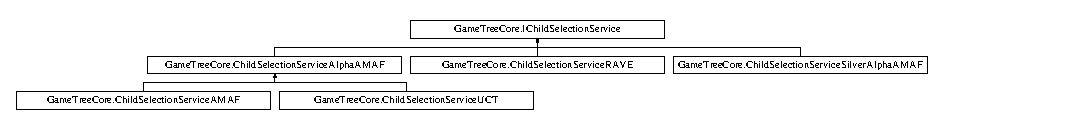
\includegraphics[height=1.242604cm]{interface_game_tree_core_1_1_i_child_selection_service}
\end{center}
\end{figure}
\subsection*{Public Member Functions}
\begin{DoxyCompactItemize}
\item 
\mbox{\Hypertarget{interface_game_tree_core_1_1_i_child_selection_service_a48cd3434b6f327de07b8522fae6d92ff}\label{interface_game_tree_core_1_1_i_child_selection_service_a48cd3434b6f327de07b8522fae6d92ff}} 
\mbox{\hyperlink{interface_game_tree_core_1_1_i_game_tree_node}{I\+Game\+Tree\+Node}} {\bfseries child\+Selection} (\mbox{\hyperlink{interface_game_tree_core_1_1_i_game_tree_node}{I\+Game\+Tree\+Node}} node, double exploration\+Constant)
\end{DoxyCompactItemize}


\subsection{Detailed Description}
Exposes a method to select a child node from a \mbox{\hyperlink{interface_game_tree_core_1_1_i_game_tree_node}{I\+Game\+Tree\+Node}}. 



Definition at line 5 of file I\+Child\+Selection\+Service.\+cs.


\hypertarget{interface_game_tree_core_1_1_i_final_child_selection_service}{}\section{Game\+Tree\+Core.\+I\+Final\+Child\+Selection\+Service Interface Reference}
\label{interface_game_tree_core_1_1_i_final_child_selection_service}\index{Game\+Tree\+Core.\+I\+Final\+Child\+Selection\+Service@{Game\+Tree\+Core.\+I\+Final\+Child\+Selection\+Service}}


Esposes a method to finally select a child node from a \mbox{\hyperlink{interface_game_tree_core_1_1_i_game_tree_node}{I\+Game\+Tree\+Node}}.  


Inheritance diagram for Game\+Tree\+Core.\+I\+Final\+Child\+Selection\+Service\+:\begin{figure}[H]
\begin{center}
\leavevmode
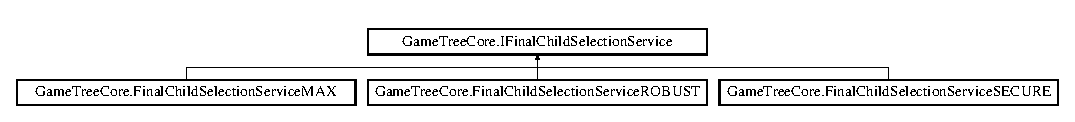
\includegraphics[height=1.196581cm]{interface_game_tree_core_1_1_i_final_child_selection_service}
\end{center}
\end{figure}
\subsection*{Public Member Functions}
\begin{DoxyCompactItemize}
\item 
\mbox{\Hypertarget{interface_game_tree_core_1_1_i_final_child_selection_service_acb0ef4792988afba065c36fe2d3811b3}\label{interface_game_tree_core_1_1_i_final_child_selection_service_acb0ef4792988afba065c36fe2d3811b3}} 
\mbox{\hyperlink{interface_game_tree_core_1_1_i_game_tree_node}{I\+Game\+Tree\+Node}} {\bfseries final\+Child\+Selection} (\mbox{\hyperlink{interface_game_tree_core_1_1_i_game_tree_node}{I\+Game\+Tree\+Node}} node)
\end{DoxyCompactItemize}


\subsection{Detailed Description}
Esposes a method to finally select a child node from a \mbox{\hyperlink{interface_game_tree_core_1_1_i_game_tree_node}{I\+Game\+Tree\+Node}}. 



Definition at line 5 of file I\+Final\+Child\+Selection\+Service.\+cs.


\hypertarget{interface_game_tree_core_1_1_i_game_tree_node}{}\section{Game\+Tree\+Core.\+I\+Game\+Tree\+Node Interface Reference}
\label{interface_game_tree_core_1_1_i_game_tree_node}\index{Game\+Tree\+Core.\+I\+Game\+Tree\+Node@{Game\+Tree\+Core.\+I\+Game\+Tree\+Node}}


Represents a node in a game tree. ~\newline
 


\subsection*{Public Member Functions}
\begin{DoxyCompactItemize}
\item 
\mbox{\Hypertarget{interface_game_tree_core_1_1_i_game_tree_node_ab5a6e0a1ba3046ecc5c79a95ca733a46}\label{interface_game_tree_core_1_1_i_game_tree_node_ab5a6e0a1ba3046ecc5c79a95ca733a46}} 
Read\+Only\+Collection$<$ \mbox{\hyperlink{interface_game_tree_core_1_1_i_game_tree_node}{I\+Game\+Tree\+Node}} $>$ {\bfseries get\+Child\+Nodes} ()
\end{DoxyCompactItemize}
\subsection*{Properties}
\begin{DoxyCompactItemize}
\item 
\mbox{\Hypertarget{interface_game_tree_core_1_1_i_game_tree_node_aa2596d50f63fa187625900043521a51b}\label{interface_game_tree_core_1_1_i_game_tree_node_aa2596d50f63fa187625900043521a51b}} 
int {\bfseries playouts}\hspace{0.3cm}{\ttfamily  \mbox{[}get\mbox{]}}
\item 
\mbox{\Hypertarget{interface_game_tree_core_1_1_i_game_tree_node_aa45086ef29ac5a68b80d3813c206369b}\label{interface_game_tree_core_1_1_i_game_tree_node_aa45086ef29ac5a68b80d3813c206369b}} 
int {\bfseries playouts\+A\+M\+AF}\hspace{0.3cm}{\ttfamily  \mbox{[}get\mbox{]}}
\item 
\mbox{\Hypertarget{interface_game_tree_core_1_1_i_game_tree_node_aaf3626012608f05f2e38b8fbfbf33523}\label{interface_game_tree_core_1_1_i_game_tree_node_aaf3626012608f05f2e38b8fbfbf33523}} 
double {\bfseries value}\hspace{0.3cm}{\ttfamily  \mbox{[}get\mbox{]}}
\item 
\mbox{\Hypertarget{interface_game_tree_core_1_1_i_game_tree_node_a5c9451b6fd10031ce6a0969f7b42d6b7}\label{interface_game_tree_core_1_1_i_game_tree_node_a5c9451b6fd10031ce6a0969f7b42d6b7}} 
double {\bfseries value\+A\+M\+AF}\hspace{0.3cm}{\ttfamily  \mbox{[}get\mbox{]}}
\item 
\mbox{\Hypertarget{interface_game_tree_core_1_1_i_game_tree_node_a14c2c88df586e02387ae50edc615b0c6}\label{interface_game_tree_core_1_1_i_game_tree_node_a14c2c88df586e02387ae50edc615b0c6}} 
bool {\bfseries are\+Child\+Nodes\+Expanded}\hspace{0.3cm}{\ttfamily  \mbox{[}get\mbox{]}}
\item 
\mbox{\Hypertarget{interface_game_tree_core_1_1_i_game_tree_node_a305c29b932bf087e19f7843c1d14e3af}\label{interface_game_tree_core_1_1_i_game_tree_node_a305c29b932bf087e19f7843c1d14e3af}} 
\mbox{\hyperlink{interface_game_tree_core_1_1_i_game_tree_node}{I\+Game\+Tree\+Node}} {\bfseries previous\+Node}\hspace{0.3cm}{\ttfamily  \mbox{[}get\mbox{]}}
\end{DoxyCompactItemize}


\subsection{Detailed Description}
Represents a node in a game tree. ~\newline




Definition at line 7 of file I\+Game\+Tree\+Node.\+cs.


%--- End generated contents ---

% Index
\backmatter
\newpage
\phantomsection
\clearemptydoublepage
\addcontentsline{toc}{chapter}{Index}
\printindex

\end{document}
